\chapter{Jaka povezanost}

\index{jako povezan graf}

U usmjerenom grafu
bridovi se mogu prijeći samo u jednom smjeru,
pa čak i ako je graf povezan,
to ne jamči da postoji
put od jednog čvora do drugog čvora.
Zbog toga je smisleno definirati novi pojam
koji zahtijeva više od povezanosti.

Graf je \key{jako povezan}
ako postoji put od svakog čvora do svih
ostalih čvorova u grafu.
Na primjer, na sljedećoj slici
lijevi graf je jako povezan,
dok desni nije.

\begin{center}
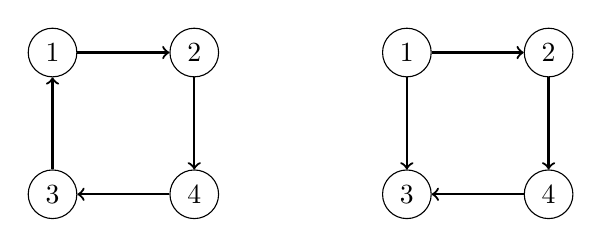
\begin{tikzpicture}[scale=0.9]
\node[draw, circle] (1) at (1,1) {$1$};
\node[draw, circle] (2) at (3,1) {$2$};
\node[draw, circle] (3) at (1,-1) {$3$};
\node[draw, circle] (4) at (3,-1) {$4$};

\path[draw,thick,->] (1) -- (2);
\path[draw,thick,->] (2) -- (4);
\path[draw,thick,->] (4) -- (3);
\path[draw,thick,->] (3) -- (1);

\node[draw, circle] (1b) at (6,1) {$1$};
\node[draw, circle] (2b) at (8,1) {$2$};
\node[draw, circle] (3b) at (6,-1) {$3$};
\node[draw, circle] (4b) at (8,-1) {$4$};

\path[draw,thick,->] (1b) -- (2b);
\path[draw,thick,->] (2b) -- (4b);
\path[draw,thick,->] (4b) -- (3b);
\path[draw,thick,->] (1b) -- (3b);
\end{tikzpicture}
\end{center}

Desni graf nije jako povezan
jer, na primjer, ne postoji put
od čvora 2 do čvora 1.

\index{komponenta jake povezanosti}
\index{graf komponenti}

\key{Komponente jake povezanosti}
grafa dijele graf na jako povezane
dijelove koji su što je moguće veći.
Komponente jake povezanosti tvore
acikličan \key{graf komponenti} koji predstavlja
dublju strukturu izvornog grafa.

Na primjer, za graf
\begin{center}
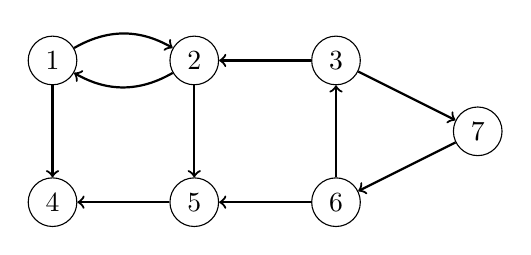
\begin{tikzpicture}[scale=0.9,label distance=-2mm]
\node[draw, circle] (1) at (-1,1) {$7$};
\node[draw, circle] (2) at (-3,2) {$3$};
\node[draw, circle] (4) at (-5,2) {$2$};
\node[draw, circle] (6) at (-7,2) {$1$};
\node[draw, circle] (3) at (-3,0) {$6$};
\node[draw, circle] (5) at (-5,0) {$5$};
\node[draw, circle] (7) at (-7,0) {$4$};

\path[draw,thick,->] (2) -- (1);
\path[draw,thick,->] (1) -- (3);
\path[draw,thick,->] (3) -- (2);
\path[draw,thick,->] (2) -- (4);
\path[draw,thick,->] (3) -- (5);
\path[draw,thick,->] (4) edge [bend left] (6);
\path[draw,thick,->] (6) edge [bend left] (4);
\path[draw,thick,->] (4) -- (5);
\path[draw,thick,->] (5) -- (7);
\path[draw,thick,->] (6) -- (7);
\end{tikzpicture}
\end{center}
komponente jake povezanosti su sljedeće:
\begin{center}
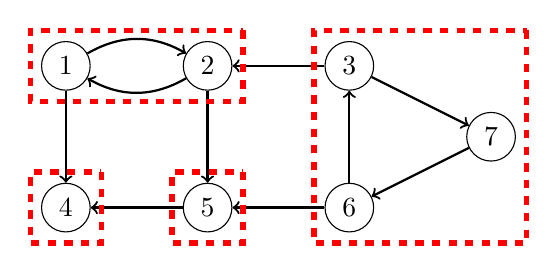
\begin{tikzpicture}[scale=0.9]
\node[draw, circle] (1) at (-1,1) {$7$};
\node[draw, circle] (2) at (-3,2) {$3$};
\node[draw, circle] (4) at (-5,2) {$2$};
\node[draw, circle] (6) at (-7,2) {$1$};
\node[draw, circle] (3) at (-3,0) {$6$};
\node[draw, circle] (5) at (-5,0) {$5$};
\node[draw, circle] (7) at (-7,0) {$4$};

\path[draw,thick,->] (2) -- (1);
\path[draw,thick,->] (1) -- (3);
\path[draw,thick,->] (3) -- (2);
\path[draw,thick,->] (2) -- (4);
\path[draw,thick,->] (3) -- (5);
\path[draw,thick,->] (4) edge [bend left] (6);
\path[draw,thick,->] (6) edge [bend left] (4);
\path[draw,thick,->] (4) -- (5);
\path[draw,thick,->] (5) -- (7);
\path[draw,thick,->] (6) -- (7);

\draw [red,thick,dashed,line width=2pt] (-0.5,2.5) rectangle (-3.5,-0.5);
\draw [red,thick,dashed,line width=2pt] (-4.5,2.5) rectangle (-7.5,1.5);
\draw [red,thick,dashed,line width=2pt] (-4.5,0.5) rectangle (-5.5,-0.5);
\draw [red,thick,dashed,line width=2pt] (-6.5,0.5) rectangle (-7.5,-0.5);
\end{tikzpicture}
\end{center}
Odgovarajući graf komponenti je sljedeći:
\begin{center}
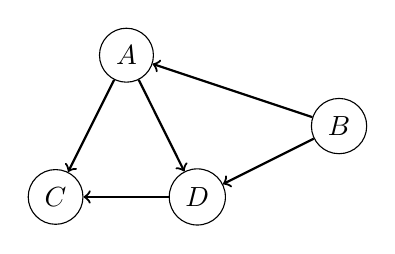
\begin{tikzpicture}[scale=0.9]
\node[draw, circle] (1) at (-3,1) {$B$};
\node[draw, circle] (2) at (-6,2) {$A$};
\node[draw, circle] (3) at (-5,0) {$D$};
\node[draw, circle] (4) at (-7,0) {$C$};

\path[draw,thick,->] (1) -- (2);
\path[draw,thick,->] (1) -- (3);
\path[draw,thick,->] (2) -- (3);
\path[draw,thick,->] (2) -- (4);
\path[draw,thick,->] (3) -- (4);
\end{tikzpicture}
\end{center}
Komponente su $A=\{1,2\}$,
$B=\{3,6,7\}$, $C=\{4\}$ i $D=\{5\}$.

Graf komponenti je acikličan usmjereni graf,
pa ga je lakše obrađivati nego izvorni graf.
Budući da graf ne sadrži ciklus,
uvijek možemo konstruirati topološko sortiranje i
koristiti tehnike dinamičkog programiranja poput onih
prikazanih u poglavlju 16.

\section{Kosarajuov algoritam}

\index{Kosarajuov algoritam}

\key{Kosarajuov algoritam}\footnote{Prema \cite{aho83},
S. R. Kosaraju je ovaj algoritam otkrio 1978.,
ali ga nije objavio. Godine 1981. isti je algoritam ponovno otkrio
i objavio M. Sharir \cite{sha81}.} je efikasna
metoda za pronalaženje komponenti jake povezanosti
usmjerenog grafa.
Algoritam izvodi dva pretraživanja u dubinu:
prvo pretraživanje konstruira listu čvorova
prema strukturi grafa,
a drugo pretraživanje tvori komponente jake povezanosti.

\subsubsection{Pretraživanje 1}

Prva faza Kosarajuova algoritma konstruira
listu čvorova u redoslijedu u kojem ih
pretraživanje u dubinu obrađuje.
Algoritam prolazi kroz čvorove
i započinje pretraživanje u dubinu u svakom 
neobrađenom čvoru.
Svaki će čvor biti dodan u listu
nakon što je obrađen.

U primjeru grafa čvorovi se obrađuju
u sljedećem redoslijedu:
\begin{center}
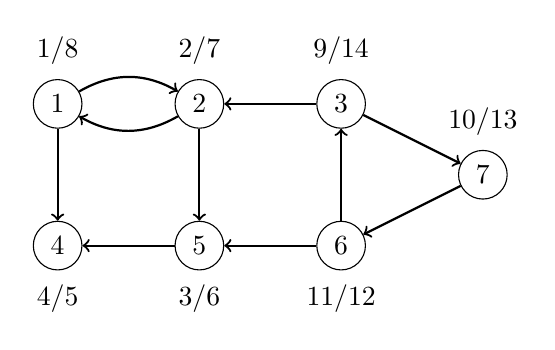
\begin{tikzpicture}[scale=0.9,label distance=-2mm]
\node[draw, circle] (1) at (-1,1) {$7$};
\node[draw, circle] (2) at (-3,2) {$3$};
\node[draw, circle] (4) at (-5,2) {$2$};
\node[draw, circle] (6) at (-7,2) {$1$};
\node[draw, circle] (3) at (-3,0) {$6$};
\node[draw, circle] (5) at (-5,0) {$5$};
\node[draw, circle] (7) at (-7,0) {$4$};

\node at (-7,2.75) {$1/8$};
\node at (-5,2.75) {$2/7$};
\node at (-3,2.75) {$9/14$};
\node at (-7,-0.75) {$4/5$};
\node at (-5,-0.75) {$3/6$};
\node at (-3,-0.75) {$11/12$};
\node at (-1,1.75) {$10/13$};

\path[draw,thick,->] (2) -- (1);
\path[draw,thick,->] (1) -- (3);
\path[draw,thick,->] (3) -- (2);
\path[draw,thick,->] (2) -- (4);
\path[draw,thick,->] (3) -- (5);
\path[draw,thick,->] (4) edge [bend left] (6);
\path[draw,thick,->] (6) edge [bend left] (4);
\path[draw,thick,->] (4) -- (5);
\path[draw,thick,->] (5) -- (7);
\path[draw,thick,->] (6) -- (7);
\end{tikzpicture}
\end{center}

Oznaka $x/y$ znači da je
obrada čvora započela
u trenutku $x$ i završila u trenutku $y$.
Prema tome, odgovarajuća lista je sljedeća:

\begin{tabular}{ll}
\\
čvor & vrijeme obrade \\
\hline
4 & 5 \\
5 & 6 \\
2 & 7 \\
1 & 8 \\
6 & 12 \\
7 & 13 \\
3 & 14 \\
\\
\end{tabular}
% 
% U drugoj fazi algoritma
% čvorovi će biti obrađeni
% u obrnutom redoslijedu: $[3,7,6,1,2,5,4]$.

\subsubsection{Pretraživanje 2}

Druga faza algoritma
tvori komponente jake povezanosti
grafa.
Prvo algoritam obrne svaki
brid u grafu.
To jamči da ćemo tijekom drugog pretraživanja
uvijek nalaziti komponente jake
povezanosti koje ne sadrže dodatne čvorove.

Nakon obrtanja bridova
primjer grafa izgleda ovako:
\begin{center}
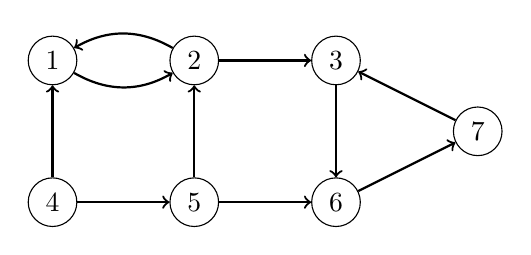
\begin{tikzpicture}[scale=0.9,label distance=-2mm]
\node[draw, circle] (1) at (-1,1) {$7$};
\node[draw, circle] (2) at (-3,2) {$3$};
\node[draw, circle] (4) at (-5,2) {$2$};
\node[draw, circle] (6) at (-7,2) {$1$};
\node[draw, circle] (3) at (-3,0) {$6$};
\node[draw, circle] (5) at (-5,0) {$5$};
\node[draw, circle] (7) at (-7,0) {$4$};

\path[draw,thick,<-] (2) -- (1);
\path[draw,thick,<-] (1) -- (3);
\path[draw,thick,<-] (3) -- (2);
\path[draw,thick,<-] (2) -- (4);
\path[draw,thick,<-] (3) -- (5);
\path[draw,thick,<-] (4) edge [bend left] (6);
\path[draw,thick,<-] (6) edge [bend left] (4);
\path[draw,thick,<-] (4) -- (5);
\path[draw,thick,<-] (5) -- (7);
\path[draw,thick,<-] (6) -- (7);
\end{tikzpicture}
\end{center}

Nakon toga algoritam prolazi kroz
listu čvorova stvorenu prvim pretraživanjem,
u \emph{obrnutom} redoslijedu.
Ako čvor ne pripada nijednoj komponenti,
algoritam stvara novu komponentu
i započinje pretraživanje u dubinu
koje sve nove čvorove nađene tijekom pretraživanja
dodaje u novu komponentu.

U primjeru grafa prva komponenta
počinje u čvoru 3:

\begin{center}
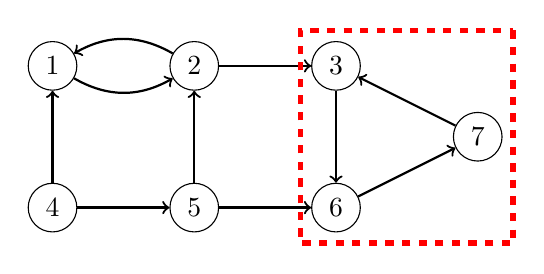
\begin{tikzpicture}[scale=0.9,label distance=-2mm]
\node[draw, circle] (1) at (-1,1) {$7$};
\node[draw, circle] (2) at (-3,2) {$3$};
\node[draw, circle] (4) at (-5,2) {$2$};
\node[draw, circle] (6) at (-7,2) {$1$};
\node[draw, circle] (3) at (-3,0) {$6$};
\node[draw, circle] (5) at (-5,0) {$5$};
\node[draw, circle] (7) at (-7,0) {$4$};

\path[draw,thick,<-] (2) -- (1);
\path[draw,thick,<-] (1) -- (3);
\path[draw,thick,<-] (3) -- (2);
\path[draw,thick,<-] (2) -- (4);
\path[draw,thick,<-] (3) -- (5);
\path[draw,thick,<-] (4) edge [bend left] (6);
\path[draw,thick,<-] (6) edge [bend left] (4);
\path[draw,thick,<-] (4) -- (5);
\path[draw,thick,<-] (5) -- (7);
\path[draw,thick,<-] (6) -- (7);

\draw [red,thick,dashed,line width=2pt] (-0.5,2.5) rectangle (-3.5,-0.5);
\end{tikzpicture}
\end{center}

Uočimo da, budući da su svi bridovi obrnuti,
komponenta ne ''istječe'' u druge dijelove grafa.

\begin{samepage}
Sljedeći čvorovi u listi su čvorovi 7 i 6,
ali oni već pripadaju nekoj komponenti,
pa sljedeća nova komponenta počinje u čvoru 1:

\begin{center}
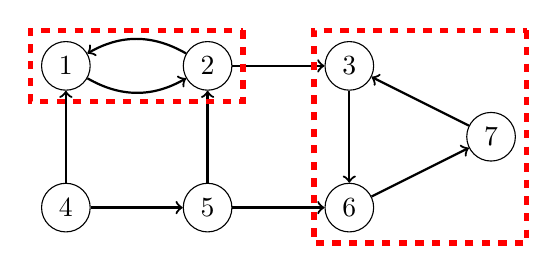
\begin{tikzpicture}[scale=0.9,label distance=-2mm]
\node[draw, circle] (1) at (-1,1) {$7$};
\node[draw, circle] (2) at (-3,2) {$3$};
\node[draw, circle] (4) at (-5,2) {$2$};
\node[draw, circle] (6) at (-7,2) {$1$};
\node[draw, circle] (3) at (-3,0) {$6$};
\node[draw, circle] (5) at (-5,0) {$5$};
\node[draw, circle] (7) at (-7,0) {$4$};

\path[draw,thick,<-] (2) -- (1);
\path[draw,thick,<-] (1) -- (3);
\path[draw,thick,<-] (3) -- (2);
\path[draw,thick,<-] (2) -- (4);
\path[draw,thick,<-] (3) -- (5);
\path[draw,thick,<-] (4) edge [bend left] (6);
\path[draw,thick,<-] (6) edge [bend left] (4);
\path[draw,thick,<-] (4) -- (5);
\path[draw,thick,<-] (5) -- (7);
\path[draw,thick,<-] (6) -- (7);

\draw [red,thick,dashed,line width=2pt] (-0.5,2.5) rectangle (-3.5,-0.5);
\draw [red,thick,dashed,line width=2pt] (-4.5,2.5) rectangle (-7.5,1.5);
%\draw [red,thick,dashed,line width=2pt] (-4.5,0.5) rectangle (-5.5,-0.5);
%\draw [red,thick,dashed,line width=2pt] (-6.5,0.5) rectangle (-7.5,-0.5);
\end{tikzpicture}
\end{center}
\end{samepage}

\begin{samepage}
Na kraju algoritam obrađuje čvorove 5 i 4
koji tvore preostale komponente jake povezanosti:

\begin{center}
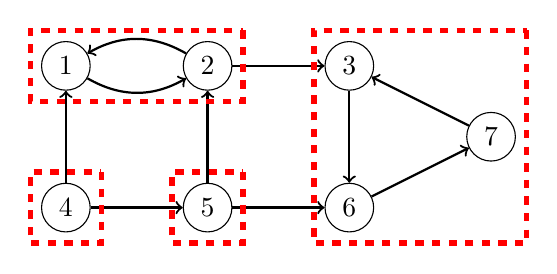
\begin{tikzpicture}[scale=0.9,label distance=-2mm]
\node[draw, circle] (1) at (-1,1) {$7$};
\node[draw, circle] (2) at (-3,2) {$3$};
\node[draw, circle] (4) at (-5,2) {$2$};
\node[draw, circle] (6) at (-7,2) {$1$};
\node[draw, circle] (3) at (-3,0) {$6$};
\node[draw, circle] (5) at (-5,0) {$5$};
\node[draw, circle] (7) at (-7,0) {$4$};

\path[draw,thick,<-] (2) -- (1);
\path[draw,thick,<-] (1) -- (3);
\path[draw,thick,<-] (3) -- (2);
\path[draw,thick,<-] (2) -- (4);
\path[draw,thick,<-] (3) -- (5);
\path[draw,thick,<-] (4) edge [bend left] (6);
\path[draw,thick,<-] (6) edge [bend left] (4);
\path[draw,thick,<-] (4) -- (5);
\path[draw,thick,<-] (5) -- (7);
\path[draw,thick,<-] (6) -- (7);

\draw [red,thick,dashed,line width=2pt] (-0.5,2.5) rectangle (-3.5,-0.5);
\draw [red,thick,dashed,line width=2pt] (-4.5,2.5) rectangle (-7.5,1.5);
\draw [red,thick,dashed,line width=2pt] (-4.5,0.5) rectangle (-5.5,-0.5);
\draw [red,thick,dashed,line width=2pt] (-6.5,0.5) rectangle (-7.5,-0.5);
\end{tikzpicture}
\end{center}
\end{samepage}

Vremenska složenost algoritma je $O(n+m)$,
jer algoritam
izvodi dva pretraživanja u dubinu.

\section{Problem 2SAT}

\index{problem 2SAT}

Jaka povezanost također je povezana s
\key{problemom 2SAT}\footnote{Algoritam prikazan ovdje
predstavljen je u \cite{asp79}.
Postoji i drugi dobro poznat algoritam linearne složenosti \cite{eve75}
koji se temelji na povratnom pretraživanju.}.
U ovom zadatku zadana nam je logička formula
\[
(a_1 \lor b_1) \land (a_2 \lor b_2) \land \cdots \land (a_m \lor b_m),
\]
gdje je svaki $a_i$ i $b_i$ ili logička varijabla
($x_1,x_2,\ldots,x_n$)
ili negacija logičke varijable
($\lnot x_1, \lnot x_2, \ldots, \lnot x_n$).
Simboli ''$\land$'' i ''$\lor$'' označavaju
logičke operatore ''i'' i ''ili''.
Naš je zadatak svakoj varijabli dodijeliti vrijednost
tako da formula bude istinita, ili utvrditi
da to nije moguće.

Na primjer, formula
\[
L_1 = (x_2 \lor \lnot x_1) \land
      (\lnot x_1 \lor \lnot x_2) \land
      (x_1 \lor x_3) \land
      (\lnot x_2 \lor \lnot x_3) \land
      (x_1 \lor x_4)
\]
istinita je kada su varijablama dodijeljene sljedeće vrijednosti:

\[
\begin{cases}
x_1 = \textrm{false} \\
x_2 = \textrm{false} \\
x_3 = \textrm{true} \\
x_4 = \textrm{true} \\
\end{cases}
\]

Međutim, formula
\[
L_2 = (x_1 \lor x_2) \land
      (x_1 \lor \lnot x_2) \land
      (\lnot x_1 \lor x_3) \land
      (\lnot x_1 \lor \lnot x_3)
\]
uvijek je neistinita, neovisno o tome kako
dodijelimo vrijednosti.
Razlog je to što ne možemo
odabrati vrijednost za $x_1$
bez da stvorimo protuslovlje.
Ako je $x_1$ neistinit, i $x_2$ i $\lnot x_2$
morali bi biti istiniti, što je nemoguće,
a ako je $x_1$ istinit, i $x_3$ i $\lnot x_3$
morali bi biti istiniti, što je također nemoguće.

Problem 2SAT može se prikazati grafom
čiji čvorovi odgovaraju
varijablama $x_i$ i negacijama $\lnot x_i$,
a bridovi određuju veze
između varijabli.
Svaki par $(a_i \lor b_i)$ stvara dva brida:
$\lnot a_i \to b_i$ i $\lnot b_i \to a_i$.
To znači da ako $a_i$ ne vrijedi,
mora vrijediti $b_i$, i obratno.

Graf za formulu $L_1$ je:
\\
\begin{center}
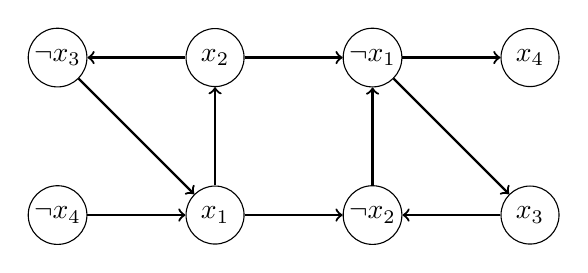
\begin{tikzpicture}[scale=1.0,minimum size=2pt]
\node[draw, circle, inner sep=1.3pt] (1) at (1,2) {$\lnot x_3$};
\node[draw, circle] (2) at (3,2) {$x_2$};
\node[draw, circle, inner sep=1.3pt] (3) at (1,0) {$\lnot x_4$};
\node[draw, circle] (4) at (3,0) {$x_1$};
\node[draw, circle, inner sep=1.3pt] (5) at (5,2) {$\lnot x_1$};
\node[draw, circle] (6) at (7,2) {$x_4$};
\node[draw, circle, inner sep=1.3pt] (7) at (5,0) {$\lnot x_2$};
\node[draw, circle] (8) at (7,0) {$x_3$};
 
\path[draw,thick,->] (1) -- (4);
\path[draw,thick,->] (4) -- (2);
\path[draw,thick,->] (2) -- (1);
\path[draw,thick,->] (3) -- (4);
\path[draw,thick,->] (2) -- (5);
\path[draw,thick,->] (4) -- (7);
\path[draw,thick,->] (5) -- (6);
\path[draw,thick,->] (5) -- (8);
\path[draw,thick,->] (8) -- (7);
\path[draw,thick,->] (7) -- (5);
\end{tikzpicture}
\end{center}
A graf za formulu $L_2$ je:
\\
\begin{center}
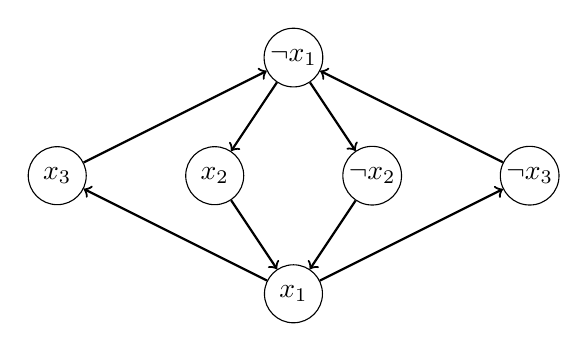
\begin{tikzpicture}[scale=1.0,minimum size=2pt]
\node[draw, circle] (1) at (1,2) {$x_3$};
\node[draw, circle] (2) at (3,2) {$x_2$};
\node[draw, circle, inner sep=1.3pt] (3) at (5,2) {$\lnot x_2$};
\node[draw, circle, inner sep=1.3pt] (4) at (7,2) {$\lnot x_3$};
\node[draw, circle, inner sep=1.3pt] (5) at (4,3.5) {$\lnot x_1$};
\node[draw, circle] (6) at (4,0.5) {$x_1$};

\path[draw,thick,->] (1) -- (5);
\path[draw,thick,->] (4) -- (5);
\path[draw,thick,->] (6) -- (1);
\path[draw,thick,->] (6) -- (4);
\path[draw,thick,->] (5) -- (2);
\path[draw,thick,->] (5) -- (3);
\path[draw,thick,->] (2) -- (6);
\path[draw,thick,->] (3) -- (6);
\end{tikzpicture}
\end{center}

Struktura grafa govori nam je li
moguće dodijeliti vrijednosti
varijablama tako
da formula bude istinita.
Pokazuje se da je to moguće
točno onda kada ne postoje čvorovi
$x_i$ i $\lnot x_i$ takvi da
oba čvora pripadaju
istoj komponenti jake povezanosti.
Ako takvi čvorovi postoje,
graf sadrži
put od $x_i$ do $\lnot x_i$
i također put od $\lnot x_i$ do $x_i$,
pa bi i $x_i$ i $\lnot x_i$ morali biti istiniti,
što nije moguće.

U grafu formule $L_1$
ne postoje čvorovi $x_i$ i $\lnot x_i$
takvi da oba čvora 
pripadaju istoj komponenti jake povezanosti,
pa rješenje postoji.
U grafu formule $L_2$
svi čvorovi pripadaju istoj komponenti jake povezanosti,
pa rješenje ne postoji.

Ako rješenje postoji, vrijednosti varijabli
mogu se pronaći prolaskom kroz čvorove
grafa komponenti u obrnutom redoslijedu topološkog sortiranja.
U svakom koraku obrađujemo komponentu 
koja ne sadrži bridove što vode u
neobrađenu komponentu.
Ako varijablama u komponenti
još nisu dodijeljene vrijednosti,
njihove će vrijednosti biti određene
prema vrijednostima u komponenti,
a ako već imaju vrijednosti,
one ostaju nepromijenjene.
Postupak se nastavlja dok svakoj varijabli
nije dodijeljena vrijednost.

Graf komponenti za formulu $L_1$ je sljedeći:
\begin{center}
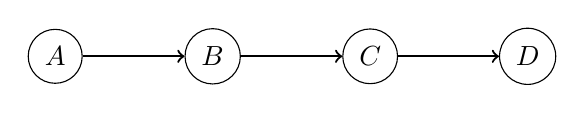
\begin{tikzpicture}[scale=1.0]
\node[draw, circle] (1) at (0,0) {$A$};
\node[draw, circle] (2) at (2,0) {$B$};
\node[draw, circle] (3) at (4,0) {$C$};
\node[draw, circle] (4) at (6,0) {$D$};

\path[draw,thick,->] (1) -- (2);
\path[draw,thick,->] (2) -- (3);
\path[draw,thick,->] (3) -- (4);
\end{tikzpicture}
\end{center}

Komponente su
$A = \{\lnot x_4\}$,
$B = \{x_1, x_2, \lnot x_3\}$,
$C = \{\lnot x_1, \lnot x_2, x_3\}$ i
$D = \{x_4\}$.
Pri konstrukciji rješenja
prvo obrađujemo komponentu $D$
u kojoj $x_4$ postaje istinit.
Nakon toga obrađujemo komponentu $C$
u kojoj $x_1$ i $x_2$ postaju neistiniti,
a $x_3$ postaje istinit.
Svim su varijablama dodijeljene vrijednosti,
pa preostale komponente $A$ i $B$
ne mijenjaju varijable.

Uočimo da ova metoda radi jer
graf ima posebnu strukturu:
ako postoje putovi od čvora $x_i$ do čvora $x_j$
i od čvora $x_j$ do čvora $\lnot x_j$,
tada čvor $x_i$ nikada ne postaje istinit.
Razlog je to što također postoji
put od čvora $\lnot x_j$ do čvora $\lnot x_i$,
pa i $x_i$ i $x_j$ postaju neistiniti.

\index{problem 3SAT}

Teži je zadatak \key{problem 3SAT},
gdje je svaki dio formule oblika
$(a_i \lor b_i \lor c_i)$.
Taj je zadatak NP-težak, pa nije poznat efikasan
algoritam za njegovo rješavanje.
